%--------------------------------------
\chapter{Implementation}
\label{chap_implementation}
%--------------------------------------

\begin{figure*}[!ht]
	\centering
    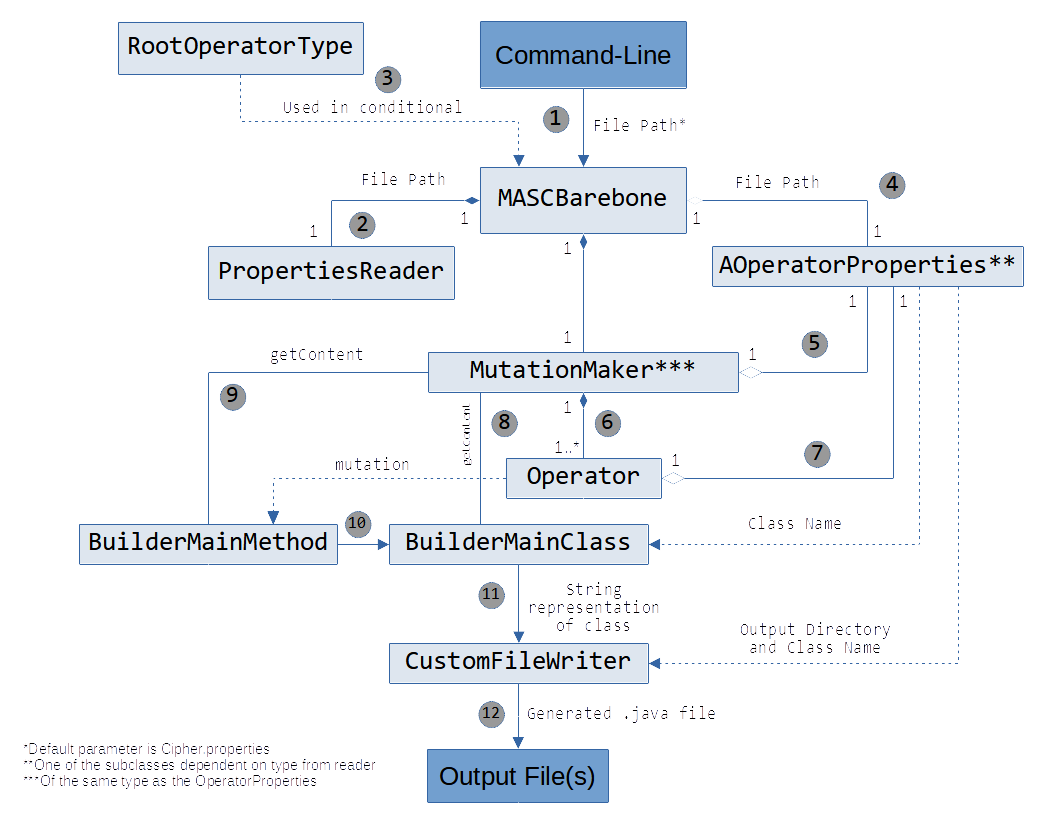
\includegraphics[width=0.96\linewidth]{figures/architecture.png}
	\vspace{-1.em}
    \caption{\small A high level diagram showing the architecture design of MASC. This further demonstrates how each component of MASC is designed and how to run the framework}
    \label{fig:taxonomy}
	
\end{figure*}

The implementation of MASC remains consist with the original work. It involves the same three original components: "(1) selecting misuse cases from the taxonomy for mutation, (2) implementing mutation operators that instantiate the miusse cases, and (3) seeding/inserting the instantiated mutants in Java/Android source code at targeted locations." The extension of the framework was build upon the foundation that was previously laid. All additions remained consistent with the implementation of the original work. A high level diagram of MASC's design is shown in Figure 3.1.

1. Selecting misuse cases from the Taxonomy: In the original work 19 misues were chosen from the taxonomy for mutation utilizing the original 12 operators. Misuses were chosen based on two main factors to ensure that different categories of cryptographic misuse were represented as well as ensuring the more prevelant cases appeared as well. For the extened work only a few additional misuse cases were added such as a static key in android keystore. However, with the expansion of the operators it possible to create many more mutants with the misuses that were already present. For this extension the previous misuses were leveraged when creating mutations. However, they were designed with other possible misuses in mind similarly to the original 12 operators.
2. Implenting mutants: The mutation operators described in the previous chapter along with the original 12 operators were desgined to be applied to one or more crypto-API, for instatiating specific misuse cases. The goal of generating mutants in programs is to ensure that they are still compilable. To ensure that this remains possible, MASC considered the necessary syntatic requirements of each API that is being implemented (such as the requirement of surrounding try-catch block with appropriate exception handling) and the semantic rrequirement of the specific misuse that is being instantiated. MASC used Java Reflection to determine all the necessary syntax to automatically create compilable mutants. After this MASC is designed to combine this component with the parameters to create the mutants.

MASC also ensures that mutants generated for evaluation are compilable using two mains steps: "(1) Using Eclipse JST's AST-based to check for identifying syntactic anomalies in the generated mutated apps, and (2) compile the mutated app automatically using build/test scripts provided with the original app." Since the portion is fully automated this is how MASC has made it possible to generate many mutants to evaluate a crypto-detector with little effort from the user.

3. Indentifying Target Locations and Seeding Mutants: To locate target locations to seed mutants using the similarity scope the MDroid+ mutation analysis project was leveraged as a component of MASC. For the original work the process it used to determine mutant locations was changed to fit the scope of MASC and support was added to include depdencies that crypto mutations introduce. When I began work on MASC this component was connected to MASC where it needed to be but contained a lot of uncessary components leftover from the original MDroid+ project that MASC was not utilizing. For the extension I identified the parts of MDroid+ that MASC was using and fully integrated them within MASC. This was done to help consolidate MASC into one project rather than a project using components from two additional projects. The components that were leveraged from MDroid+ still exist but now are fully integrated within MASC.

Similarly MASC also extended µSE to create the exhaustive scope. The extended µSE was used to find locations where crypto-APIs can be insterted in a program and still allow the program to be compilable. Just like MDroid+ I integrated the parts of µSE that MASC utilized into the main program. 

In addition the same flaw of corner cases with mutants causing compliation errors still exists within MASC. Due to how MASC is implemented this is something that is not easy to change. These cases still have a change to appear in 0.098\% of cases.


%--------------------------------------
\subsection{New Features}
\label{ch3:sec:new-features}
%--------------------------------------

While many of the new additions to MASC came in the form of extending work that was already there and heavily extended the evaluation. I also introduced a couple of new features into MASC to help make the framework more user friendly and allow a new perspective of evaluation to be conducted.

%--------------------------------------
\subsection{Sensitivity Evaluator}
\label{ch3:subsec:sensitities}
%--------------------------------------

The sensitivity evaluator is a new component of the MASC framework designed as an alternative way for users evaluate crypto-detectors. This tool is designed to help users access the oprators without having to understand the specifics of what each operator does. In security analysis there are sensitivities that are commonly discussed in relation to static analysis tools. These crypto-detectors are built with these sensitivities in mind and claim to be able to logically handle some of them. The main sensitivities I found when look through past work were flow sensitivity, alias sensitivity, context sensitivity, path sensitivity, and object sensitivity. For this work the sensitivities are defined as the following:

Flow Sensitivity - Flow sensitivity is an incredibly precise form of sensitivity. It recognizes the order that statements are performed and can keep track of the state of the program at that point in time. A flow sensitive analysis performs its analysis based on the sequence of statements. It can tell if two variables are assigned after line 23 while a flow insensitive analysis will only know that the two variables were assigned at some point within the scope of their analysis. A flow analysis will only take into consideration portions of the program that would be run based on the previous lines. Flow sensitivity analysis is a extremely expensive computationally.

Alias Sensitivity - Alias sensitivity is typically a variation of context or flow sensitivity. In Java alias sensitivity is typically type based, this is because Java is a type safe language. Alias sensitivity is the ability to keep track of a variable that has been aliased to another variable and still keeping track of the value. If there is a variable named x that equals 1 and we pass this into a method this passed value would be an alias of x.

Context Sensitivity - Context sensitivity takes into account the information throughout the program when method calls are made to determine if there is a vulnerability. It can differentiate between two different function calls to the same method with different variables. A context insensitive approach would flag both function calls if one of them was considered vulnerable while a context sensitive approach can differentiate between the two calls. A less sophisticated version of this is interprocedural sensitivity.

Path/Conditional Sensitivity - Path sensitivity only takes into consideration paths through the program that are feasible. It has a heavy focus on things such as conditionals. Within programs some paths or statements can not be reached by the code, a path sensitive analysis would not flag a vulnerability that is unreachable. Path sensitive analysis is only concerned with the path of the program that is possible to be executed.

Field/Index Sensitivity - Field sensitivity is the ability to differentiate different fields that are a part of the same object. If an object contains two variables one tainted and one that is not tainted and the non tainted one is called a field sensitive analysis would not flag the object as a vulnerability. This requires keeping track of all the contents of objects separately and understanding when certain aspects of an object are called by the program.
    
Object Sensitivty - Object sensitivity takes into account different versions of the same object. It has the ability to understand the difference between a version of an object that contains a vulnerability and one that does not contain a vulnerability. If we create two versions of object FOO called f1 and f2 and place a vulnerability in f2 but only interact with f1, an object sensitive tool would be able to recognize that there is not vulnerability taking place.

With these definitions in mind for the sensitivities I designed the sensitivity evaluator. This tool allows MASC to be run and generate mutants that fit into each specified definition. Once these definitions were clearly defined, I categorized each operator into the category or categories that it fit under. Then with this knowledge I designed the sensitivity runner so that MASC would only produce output based on a specified sensitivity. This was done to lower the barrier of entry for MASC as well as create a new way of evaluting crypto-detectors using MASC. By defining operators in this way it is possible to put more emphasis on cases that fit the description of a crypto-detector. If a crypto-detector made a claim that it was flow sensitive now it is possible to easily run all the cases that are defined to be flow sensitive and see how well it performs against those mutants instead of trying to determine which operators might fit this definition. It would be expected that a crypto-detector that claims to handle a certain sensitivity would be better suited to handle those cases. 

The sensitivity evaluator combines the input of all of the various cases and allows the user to specify how they want to run it in one file. It then handles creating all the operators that are related to the selected sensitivity. It will create the operators with the parameters provided by the user within each operator. This tool should make MASC more accessible to those with some knowledge of security without having to get a full grasp about how the operators and specifics of MASC work. I believe both the user interactivity aspect of this and the new perspective will be greatly beneficial to performing the research. Currently, it only creates minimal examples but was designed to easily be exapnde to the other scopes.


%--------------------------------------
\subsection{Automated Evaluation}
\label{ch3:subsec:automation}
%--------------------------------------

In the original paper all analysis from all the crypto detectors was done by hand so it required many man hours and double checking to ensure there were no errors. To help determine results for researchers and users an additional tool was created for MASC. This tool is the automated analysis. This allows researchers to run MASC on certain crypto detectors and MASC will automatically parse the results and let the user know if the crypto detector failed and how it failed. This tool can also take output from various crypto detectors that were given MASC code and can tell where the crypto detector failed. This is done using a SARIF parser that was created. SARIF stands for Static Analysis Results Interchange Format. This file format is becoming the standard output for Static Analysis tools and is being pushed heavily by GitHub. At the time of creating this tool this file format was fairly new and did not have many tools created to parse its contents. To build the automated analysis component it required first to build a tool that could parse the SARIF format. SARIF format shares a lot of similarities with JSON so I leveraged some Java JSON libraries such as the Google JSON simple library. I built a SARIF layer on top of this library to create a tool for parsing output. The SARIF parser tool I created takes in two SARIF files as input one of the code before mutation that was passed into the crypto detector and one Sarif file that was mutated and seeded with misuses. This is done so that if there were any misuses present in the program before MASC was run that are not taken into account and added to the total of misuses the crypto detector found because of MASC. 

More specifically, I created a tool that is able to parse a SARIF output from a Crypto-API Misuse Detector to determine which seeded misuse cases were caught by the detector.  Put another way, this component checks to make sure the Crypto-API Misuse Detectors were actually able to catch the misuses seeded in the program. Currently, this tool only works for the Main scope of the MASC Framework.  However, it can easily be expanded to work with the Exhaustive and Selective scopes in the next extensions of the MASC Framework. 
    
In terms of how the tool works, it takes the SARIF output files obtained from the Crypto-API Misuse Detectors as input along with the MASC properties file used for mutation. Using this information the tool parses through the MASC properties file to determine where the created mutated Java files were placed and what the Crypto-API name is being tested.  Using this information, the mutated Java files that were created are scanned to find the line that contains the misuse.  Once the misuses are found it is then possible to scan through the results of the SARIF file using Flow Analysis.

Flow Analysis in terms of how it is used in this project is the idea that each misuse created by an operator can be represented as a different level of complexity.  MASC inherently has levels of complexity already designed into it. To put it simply, a Crypto-API Misuse Detector will have an easier time catching a misuse like “AES” than “A$\sim$ ES”.replace(“$\sim$”,””) since the former example is less syntactically complex than the latter example. By designing it this way, the SARIF files can then be analyzed in order of complexity starting with the most basic misuse (or “base case” misuse) and increasing to the more complex ones until the Crypto-API Misuse Detector fails to catch one. If the crypto-detector fails then the analysis can stop because if a tool cannot find a less complex misuse it would not be expected to find a more complex or mutated misuse case.  Implementing the evaluator in this way makes it a lot easier to determine where Crypto-API Misuse Detectors fail and saves a lot of manual effort since this can all be done in an automated fashion.  This process also reduces the risk created by manual evaluation. 

The tool was later expanded and used a part of the main MASC properties file. It was made possible that when MASC was run it could run the output it creates against a Crypto Detector check that output and let the user know which mutants were found. This additional step was built on top of the SARIF Parsing tool to create the full end to end automated analysis. This step was the integration of the SARIF Parsing analysis tool with the entire main project since the original tool looked at outputs of crypto detectors that had MASC mutants run on them. The new full automated analysis takes that work and brings together with MASC being run as well combines crypto-dectors such as CogniCrypt by running it as a part of the analysis.

Both the SARIF parsing tool and the combination with automated analysis should help users as well as researchers save a lot of time when examining crypto-detectors. This automated analysis is less error prone and can help automatically determine if a mutation was caught but also what the likely cause of the failure was. It can determine with its Flow Analysis what level of complexity caused the failure and help more easily identify the potential flaws found within detectors. Overall the tool helps MASC become a more complete project and continues to make it more accessible. This helps to further MASC’s goal of improving crypto-detectors by better identifying exactly where they fail. 

%--------------------------------------
\subsection{MASC Web}
\label{ch3:subsec:web}
%--------------------------------------

In another attempt to make MASC user friendly. I designed the initial version of a website for MASC. Currently a second version of MASC Web is in active development using Django instead of Flask (which was originally used). The goal of the website was to introduce users to MASC and allow them to mutate files directly on the website. I integrated MASC into the website and made it so users could upload a file and specify the parameters they wanted mutated as well as the operator they wanted to use. The website would then provide them with both the original version and the mutated version of the file. Eventually, the goal is to deploy the website to help increase visibility of MASC and allow for additional options for users to access MASC.

